\documentclass[a4paper]{scrartcl}

\usepackage{authblk}

\usepackage[USenglish]{babel}

\usepackage{bibentry}
\usepackage[official]{eurosym}

\usepackage{enumitem}

\usepackage[T1]{fontenc}

\usepackage{graphicx}

\usepackage{hyperref}

\usepackage[utf8]{inputenc}

\usepackage{longtable}

\usepackage{lscape}

\usepackage{minted}

\usepackage{todonotes}

\usepackage{verbatim}

\newcommand{\seeUrl}[1]{\footnote{See \mbox{\url{#1}}}}
\newcommand{\textt}[1]{{\small \texttt{#1}}}

\setlist{nolistsep}

% Disable default paragraph indentation.
\setlength{\parskip}{\baselineskip}
\setlength{\parindent}{0cm}

\title{Modern Ways of Spatial Data Publication}
\author{Wouter Beek ({\small\url{wouter@triply.cc}})}
\author{Laurens Rietveld ({\small\url{laurens@triply.cc}})}
\affil{Triply ({\small\url{http://triply.cc}})}

\begin{document}

\maketitle

\begin{abstract}
  \noindent Almost every interesting dataset has some spatial
  component.  Besides being prevalent, spatial relations --
  particularly geographical ones -- tie the online to the offline
  world.  As such, they provide a grounding of data stored in
  databases to the physical environment that is described in those
  databases.

  Given the availability of Semantic Web services, Linked Datasets and
  Open Source web libraries we should be able to build a demonstration
  system that allows web programmers to build innovative applications
  on top of integrated Linked (Geo)datasets.  Unfortunately, we found
  out that this is not (yet) the case.
\end{abstract}


\section{Introduction}

Earlier research by GeoNovum has resulted in a collection of lessons
learned that describe in great detail the requirements of a modern
spatial data publishing infrastructure.  The purpose of the present
report is to document our research findings based on this prior work
in an attempt to answer the following research question:

\begin{quote}
  How do the lessons learned meet the constraints (e.g., budgets) and
  capabilities (e.g., in-house know-how) of governmental organizations
  on the one hand, and of data users on the other?
\end{quote}

While every governmental organization will be different, e.g., will be
required to follow different rules and regulations depending on the
domain or context in which it operates, it is possible to quantify the
investment needed in order to build a Linked Geodata platform that
implements the lessons learned.

In addition to describing and quantifying the effort required to meet
the constraints laid down in the existing lessons learned, we also
describe the problems of publishing Linked Geodata in general.
According to our assessment there are no off-the-shelf tools that
allow Linked + geospatial data to be queried with acceptable
performance.


\begin{comment}
\section{Approach}

Quantification is performed in a four-stage process:

\begin{itemize}

\item Information gathering: Based on Linked Data and Geodata experts
  and available we perform a quick information gathering round in which
  we form an overview of the directions we can take in order to answer
  our research question.  The information gathered is not intended to
  be complete but is intended to give a global direction for
  subsequent stages.  A more extensive information gathering approach
  may be undertaken in the future.

\item Scaffolding step: Based on the information gathered, we make an
  assessment of current platforms, libraries and tools that would
  allow the requirements to be implemented.  Also, some of the
  strengths and weaknesses that did not surface during the information
  gathering stage may come up here.

\item Filling in the blanks: Not all requirements may be available
  from off-the-shelf tools.  It may therefore be necessary to develop
  the remaining requirements.  This can either be done as a community
  effort or by the organization itself.  The cost/benefit calculations
  for these two approaches are very different: while the costs of a
  community effort can be spread and are therefore generally lower,
  development may take a while.  On the other hand, in-house
  development is relatively expensive but is likely to result in a
  quick first working solution.  In practice, the challenge is to turn
  components that are developed in-house for speed into long-running
  community projects afterwards.

\item Test \& iterate: Once an acceptable platform is assembled we
  need to go through several iterations of testing, upgrading and
  testing.  We were not able to reach this fourth step in this
  research.  Section~\ref{sec:conclusion} gives details as to why.

\end{itemize}
\end{comment}

% Lesson 1C: Think carefully about who is allowed to do what
% Lesson 1D: Each speaks its own language and lives in his own world

\subsection{Primary use case}
\label{sec:use_case}

Primary use case: proximity queries


\section{Storage}
\label{sec:storage}

\begin{quote}
  Do not use existing WoD products to implement a Web-based geospatial
  stack.
\end{quote}

The first choice we have to make is how we want to store Linked
Geospatial data.  This choice has repercussions for almost all other
aspects of the system, e.g., which queries can be performed and how
long it takes to answer them.


\subsection{First strategy: use a SotA triple store}

Our first intuition was that SotA triple stores would be able to
support geospatial data quite well.  We were wrong in this.  We first
determined the leading query paradigm for geospatial Linked Data: this
is GeoSPARQL~\cite{Battle2011}.  We then determined the tool with the
best GeoSPARQL support: this is
Virtuoso\seeUrl{https://github.com/openlink/virtuoso-opensource}.  We
  have loaded the data into an endpoint running version 7.2 (March
  2016) hosted at \url{http://sparql.geonovum.triply.cc/sparql}.

Unfortunately, Virtuoso does not support all geometries.  Our data
contains curves, resulting in the following error whenever a curve is
encountered by the query engine:

\begin{minted}{text}
  Virtuoso 42000 Error GEO..: for after check of geo intersects, some
  shape types (e.g., polygon rings and curves) are not yet supported
\end{minted}

Here is an example of a query that gives the above warning (``pairs of
intersecting geometries that belong to the same resource''):

\begin{minted}{sparql}
PREFIX geo: <http://www.opengis.net/ont/geosparql#>
SELECT ?y1 ?y2
WHERE {
  ?x geo:asWKT ?y1 .
  ?x geo:asWKT ?y2
  FILTER (bif:st_intersects (?y1, ?y2, 0.1))
}
\end{minted}

A second issue is that some queries do not terminate at all, as
indicated by the following message:

\begin{minted}{text}
  Virtuoso S1T00 Error SR171: Transaction timed out
\end{minted}

An example is an altered version of the previous query (``five pairs
of dissimilar intersecting geometries that belong to the same
resource''):

\begin{minted}{sparql}
PREFIX geo: <http://www.opengis.net/ont/geosparql#>
SELECT ?y1 ?y2 {
  ?x geo:asWKT ?y1 .
  ?x geo:asWKT ?y2
  FILTER (bif:st_intersects (?y1, ?y2, 0.1) && ?y1 != ?y2)
}
LIMIT 5
\end{minted}

Thirdly, not all combinations of supported functions and supported
shapes are supported.  For instance, the following implements the
query for our primary use case:

\begin{minted}{sparql}
PREFIX geo: <http://www.opengis.net/ont/geosparql#>
SELECT ?y (MIN(bif:st_distance(?y, bif:st_point(0, 52))) AS ?z)
WHERE {
  ?x1 geo:asWKT ?y
}
LIMIT 5
\end{minted}

In this particular case, the problem is that distance can only be
calculated between points but not between a point and a surface, as
communicated by the following message:

\begin{minted}{text}
Virtuoso 22023 Error GEO..: Function st_distance() expects a geometry
of type 1 as argument 0, not geometry of type 10242
\end{minted}

The fourth and biggest problem is that queries that combine geo
functions and graph relations take \emph{very} long to compute.  For
testing purposes we have set the limit for query execution to 10,000
seconds, but some queries still do not succeed within that time-frame:

\begin{minted}{text}
  Virtuoso 42000 Error The estimated execution time 12774 (sec)
  exceeds the limit of 10000 (sec).
\end{minted}

We must note that both Virtuoso and StarDog are very good triple
stores overall and that they are working on improving geodata and
GeoSPARQL support.  It is difficult to assess when those improvements
will be good enough to sufficiently support geospatial data
publication.


\subsection{Second strategy: use a SotA Information Retrieval solution}

We have corroborated our findings about the deficiency of existing
triple stores with other developers.  One common approach is to
perform graph queries in a triple store and geospatial queries in a
document store such as Solr\seeUrl{http://lucene.apache.org/solr/}.
This approach results in a good performance and coverage for
graph/SPARQL queries as well as good performance and coverage for
geospatial queries.  However, because the results come form two
disconnected backends, it is generally not possible to efficiently
perform a GeoSPARQL query in which graph and geospatial components are
intertwined.  Unfortunately, it is precisely in these integrated
queries that the benefits of using Linked Data will become apparent
(Section~\ref{sec:use_case}).


\subsection{Third strategy: use SotA GIS libraries}

Concluding that the previous two strategies will not result in a
satisfactory spatial data publication platform, we decided to go for
an out-of-the-box approach by looking beyond common Linked Data
practices.  We asked GIS experts what they use.
PostGIS\seeUrl{http://postgis.net/}, based on the
PostgreSQL\seeUrl{https://www.postgresql.org/} database, was
unanimously considered the most performant tool for handling
geospatial data.  Other tool that was mentioned was
qGIS\seeUrl{http://qgis.org/en/site/}, an Open Source GIS.  Both tools
use the backend library GEOS\seeUrl{https://trac.osgeo.org/geos}.

Our reasoning was that if PostgreSQL could be successfully combined
with GEOS that we should be possible to combine a triple store with
GEOS as well.  In fact, we found a 6 year old research
paper~\cite{VanHage2010} that had attempted to do the same thing.  The
paper had combined GEOS as a plugin of
ClioPatria~\cite{Wielemaker2015}, a triple store that we happened to be
familiar with.


\section{Communities have different needs \& capacities (Lesson 1)}
\label{sec:result_set_formats}

One of the ways in which multiple groups of users can be addressed is
by offering result set formats that they are familiar with.  Our
demonstrator exposes the following result set formats:

\begin{itemize}

\item GeoJSON

\item JSON-LD 1.0

\item N-Quads 1.1, N-Triples 1.1

\end{itemize}

N-Quads and N-Triples are, implementation-wise, the simplest RDF
serialization formats available.  They are supported by almost every
RDF processor.  Additional RDF serialization formats like Turtle 1.1,
RDF/XML 1.1 and TRiG 1.1 are also widely available and are easy to
add.  We notice that the JavaScript RDF libraries\footnote{For more
  information, see the RDF JavaScript Libraries Group
  (\url{https://www.w3.org/community/rdfjs/}).} that are currently
developed for client-side processing do not support, and will maybe
never support, RDF/XML.


\subsection{Header Dictionary Triples (HDT)}
\label{sec:hdt}

Another format that could be added is Header Dictionary Triples
(HDT)~\cite{Fernandez2013}.  These are currently used to power the
Graph API to allow Basic Graph Pattern queries to be performed
(similar to Linked Data Fragments (LDF)~\cite{Verborgh2014}).  This
format could be interesting for users who want to gather very large
result sets.

Textual serialization formats work well for small results sets.  For
instance, if someone asks the ten nearest monuments then this can
easily be returned in a text-based reply.  However, some users have a
large-scale use case, such as requesting \emph{all} monuments in the
Netherlands (e..g, with the purpose of data visualization) A textual
result set of this size is difficult to process.  With HDT the data is
not only much smaller in size (as with regular compression) but can
also be easily processed by the user.


\subsection{JSON-LD}
\label{sec:jsonld}

JSON-LD 1.0 support was the most problematic result format to
implement.  It differs from Turtle-based serialization formats in that
it does not translate a graph to a sequence of characters, but it
instead performs transformations between RDF graphs and JSON trees.
As such it has to merry requirements from both paradigms.  In this
sense JSON-LD is similar to RDF/XML which undertakes a graph to/from
tree mapping as well.

JSON-LD is valid JSON, the primary data interchange format for web
programmers.  As such, JSON-LD is a good way of lowering the entry
level for this user group.  The JSON-LD format is relatively costly to
generate and process, because not all aspects of RDF can be directly
encoded in JSON.  For this a \emph{context} that steers the data
transformation step needs to be defined (while generating) and applied
(while processing).  However, as long as JSON-LD is used for
interchanging smaller chunks of data, the extra processing time is not
an issue.

There are currently JSON-LD implementations for C\#, Go, Java,
JavaScript, PHP, Python, Ruby.  Most notably support for C and C++,
languages, in which many low-level database systems and libraries are
written, is missing.  Sadly, the top C++-based RDF processor,
Raptor\seeUrl{http://librdf.org/raptor/}, states on its web site that
``JSON-LD is not supported - too complex to implement''.

Virtuoso does not support loading JSON-LD
files\seeUrl{https://github.com/openlink/virtuoso-opensource/issues/478}
and ClioPatria does not support JSON-LD out-of-the-box either.  We
have written a partial implementation for generating JSON-LD and
included it into library plRdf\seeUrl{https://github.com/wouterbeek/plRdf/blob/master/prolog/jsonld/jsonld_build.pl}.


\subsection{GeoJSON}
\label{sec:geojson}

Another format we expose is GeoJSON.  The GeoJSON format is not yet
fully standardized\footnote{GeoJSON is a proposed RFC standard as of
  August 2016.} and the current RFC~\cite{Butler2016} is not a
standard in the traditional sense of the word, i.e., a definition of
all and only GeoJSON constructs and their meaning.  For instance, the
current RFC does not give a formal grammar but relies on examples to
convey GeoJSON syntax and semantics.

An important difference with JSON-LD is that GeoJSON cannot be read
back as Linked Data.  As a consequence, GeoJSON should only be used in
very specific circumstances.  E.g., as an export format for
applications that do not understand Linked Data, like
Leaflet\seeUrl{http://leafletjs.com}.  If a Linked Data-capable
application accesses the data in GeoJSON it is unnecessarily throwing
most of the RDF semantics away.

It is not difficult to implement GeoJSON, which is a very flexible
format that can easily be combined with other JSON formats.
Specifically, we were interested in mixing GeoJSON into JSON-LD
constructs.  This would make it a viable format for Linked Data and
non-Linked Data applications alike.  Some people have worked on this
in 2015 under the name
`geojson-ld'\seeUrl{https://github.com/geojson/geojson-ld}, but
development in that direction has now stalled.

The biggest hurdle towards integrating GeoJSON and JSON-LD into one
format is that JSON arrays are used in JSON-LD for abbreviated object
term notation.  However, GeoJSON uses JSON arrays to represent
geometries (nested lists of floating point coordinates).  This point
will be addressed in JSON-LD
1.1\seeUrl{https://github.com/json-ld/json-ld.org/issues/397}.


\subsection{OGC standards (GML, WFS, WMS)}
\label{sec:ogc}

While GeoJSON addresses users from the web and geo domain, it may not
address more advanced GIS users who may want to use more comprehensive
formats standardized by the OGC.  These formats include GML, WFS and
WMS.  The cost of integrating these OGC formats into a Linked Data
platform are considerable, because they have their own vocabularies
that need to be mapped to and from RDF.  Luckily, the OGC and W3C are
currently working on integrating their respective standards within the
Spatial Data on the Web Working
Group\seeUrl{https://www.w3.org/2015/spatial/wiki/Main_Page}.  It is
probably a good idea to wait until that Working Group has come up with
a first (proposed) standard.


\section{Findability (Lesson 1A)}
\label{sec:findability}

One of the most difficult things for users of a Linked Geodata
service, is to find out \emph{what is in the data}.  We distinguish
between the problem of finding out what the vocabulary is
(Section~\ref{sec:vocabulary_overview}) and finding out which
instances are described in the data
(Section~\ref{sec:instance_findability}).  A user often needs to know
what is in the vocabulary, in order to be able to write a query to
find particular instances.


\subsection{Vocabulary overview}
\label{sec:vocabulary_overview}

It is difficult to gain an overview of a Linked Data vocabulary.  For
non-Linked Data services this is usually not a problem: there is a
limited number of entity types and relations that can be queried.  For
instance, a product review site may have users who write reviews for
products.  Products may have companies producing them and users may
themselves have ratings to denote their trust level.  That's about it.

Linked Data is very different: the RCE monument dataset contains over
a hundred unique relationships between entities belonging to dozens of
different types.  And this is only one dataset.  It is inherently
difficult to provide an overview of what is inside a large collection
of Linked Data, in the same way in which it is impossible to provide
an overview of what is in a large collection of the web.

\textbf{Hierarchy visualization} can be used to display the class
and/or property hierarchy in a tree view.  E.g., StarDog successfully
uses this in their default data browser.

\textbf{Domain/range visualization} can be used to display the classes
and properties in relation to each other.  Value properties are
displayed as part of the class nodes.  Object properties are displayed
as directed arcs between class nodes.  This requires domain
(\textt{rdfs:domain}) and range (\textt{rdfs:range}) information for
the properties.  Figure~\ref{fig:vocab_viz} shows an example for the
Semantic blogging platform SemBlog.

\begin{figure}
  \centering
  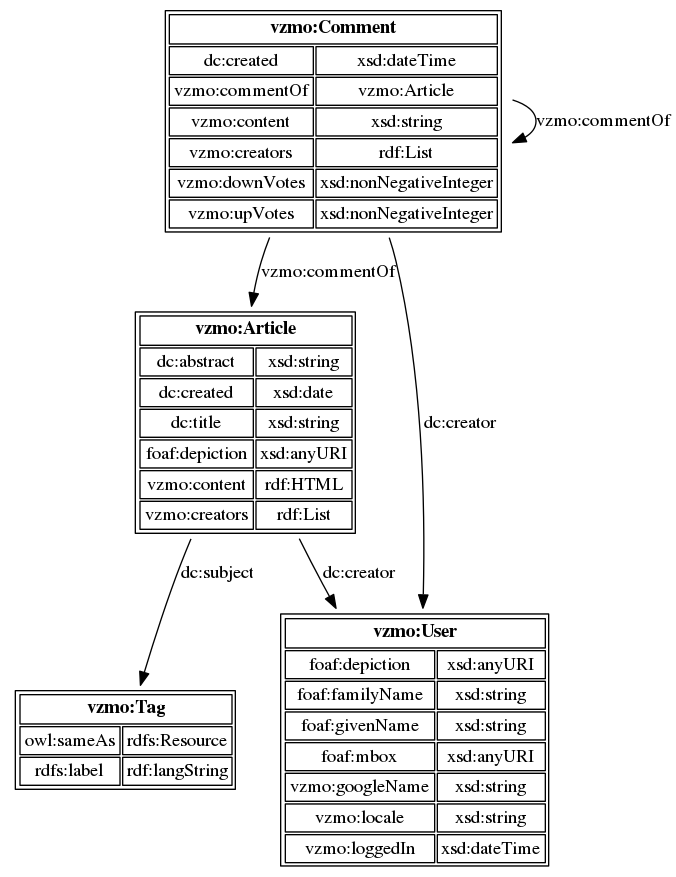
\includegraphics[width=0.75\linewidth]{img/vocab_viz}
  \caption{Example of a vocabulary visualization with 4 classes, 5
    object properties, and 20 value properties.}
  \label{fig:vocab_viz}
\end{figure}

If OWL cardinality restrictions are also present then this can also be
used to annotate the arcs.  We are unaware of a tool that does this
currently, but in theory it should be possible to generate
visualizations that are somewhat akin to class diagrams in
object-oriented software engineering (e.g., UML class diagrams).

Unfortunately, our source datasets (Section~\ref{sec:source_data})
contain very little hierarchical information and no domain/range
information.  In order for existing visualization techniques to be
applicable we have to first perform a data enrichment operation.  Data
that is automatically converted from non-RDF formats will often lack
this information.

\paragraph{Cost}
The cost of vocabulary visualization are low when the data contains
sufficient hierarchical and/or domain/range information.  Otherwise,
the cost of adding such schema information to the dataset is
relatively high.


\subsection{Instance findability}
\label{sec:instance_findability}

Datasets can be very large, so good search functions are required to
let users find the needle in the haystack.  There are two main
approaches towards finding instances in Linked Datasets.  The former
is based on \textbf{text-based search}, which uses techniques from
Information Retrieval (IR) to perform string matching in combination
with relevance ranking.  We implemented a simple text-based search
feature that indexes all RDF literals and matches substrings against
them.

Figure~\ref{fig:search} shows the results for searching for the
`Hofnar' building.  One result is the building as described by the
BGT.  Another result is a strike event that took place at the Hofnar
building in 1979, where 24 workers demanded higher wages.  The
remaining result is unrelated, it is a monument with a depiction of a
jester (`hofnar' in Dutch).

\begin{figure}
  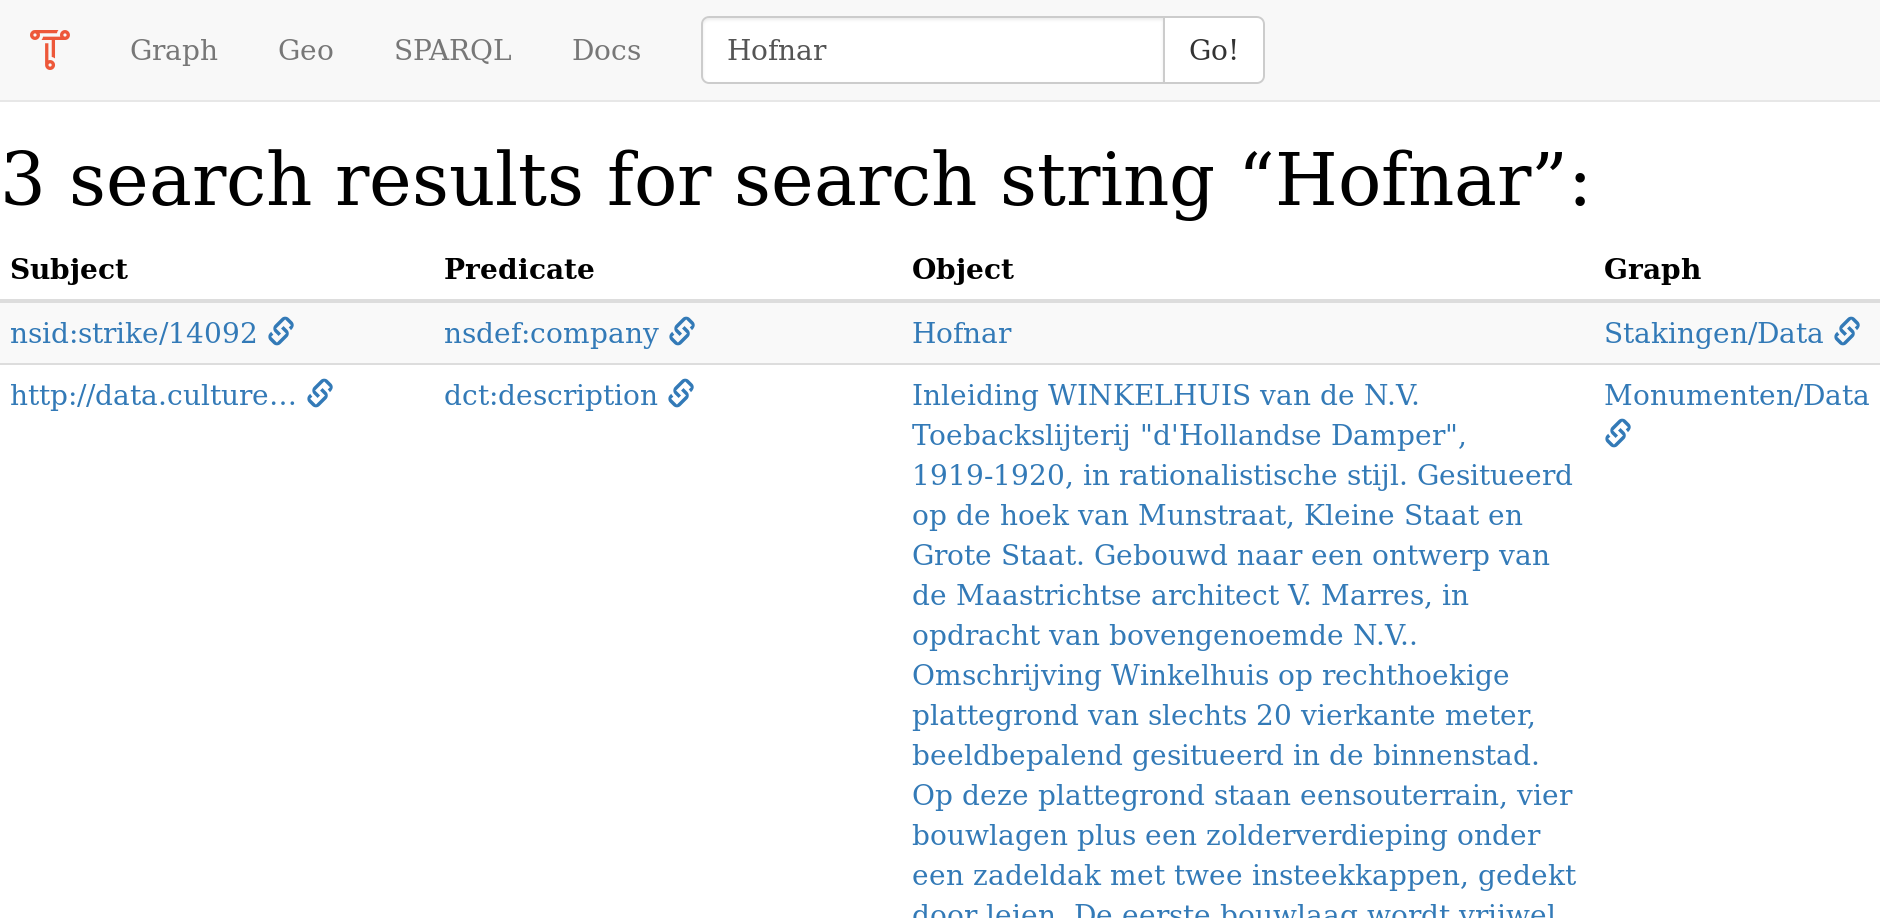
\includegraphics[width=\linewidth]{img/search}
  \caption{Results for the search ``Hofnar''.}
  \label{fig:search}
\end{figure}

What is currently lacking is a good ranking over the matched results.
This would put resources called `Hofnar' higher in the search results
than resources that only contain the word somewhere in a lengthy
description.  Better search results are obtained by using a dedicated
IR backend like ElasticSearch/Lucene.\footnote{An example of an
  ElasticSearch deployment over Linked Data is our LOD~Search
  (\href{http://lodsearch.org}) endpoint that indexes 4.3 billion
  literals.}

The second approach for finding instances in Linked Data is not based
on string matching but on the structure of the vocabulary.  It is
implemented in \textbf{faceted browsers} that allow classes and
properties to be selected from automatically generated option lists.
By selecting options from these lists the user applies filters to the
dataset, resulting in an increasingly smaller results set of entities
that adhere to the specified filters.  A screenshot of a faceted
browser is shown in Figure~\ref{fig:faceted_browser}.

\begin{figure}
  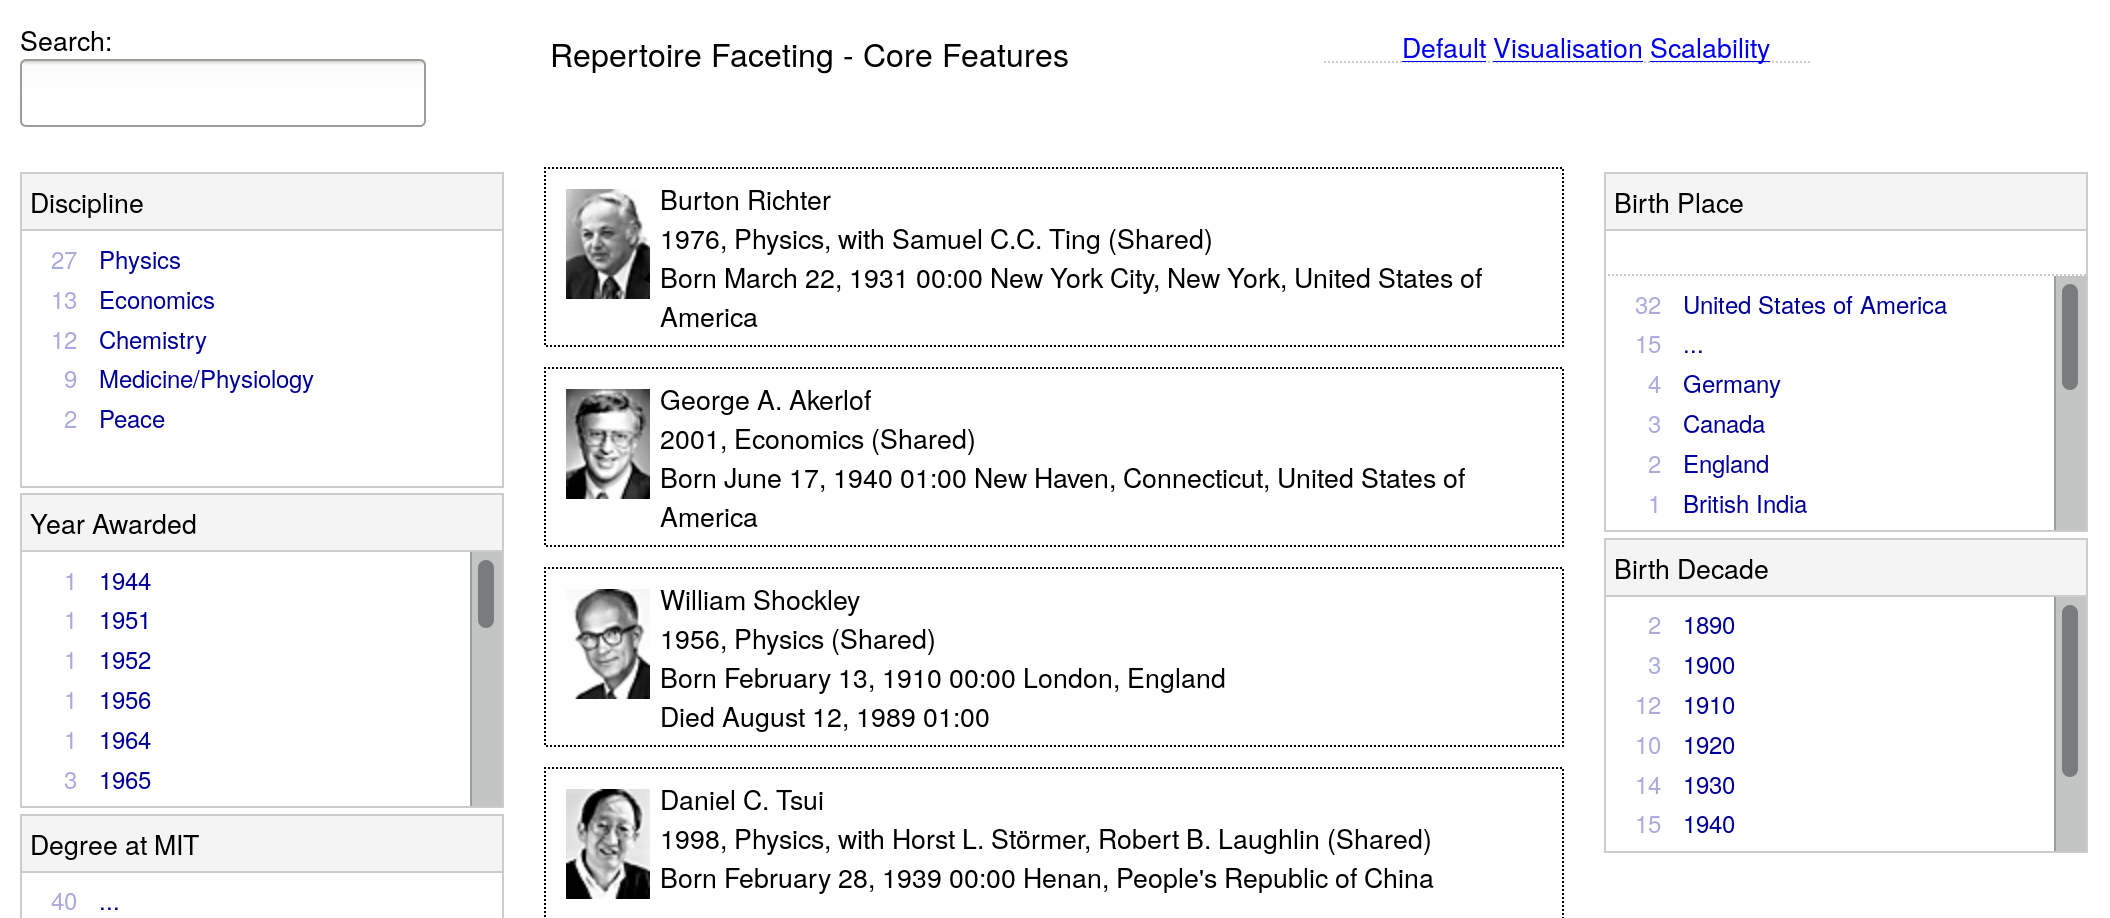
\includegraphics[width=\linewidth]{img/faceted_browser}
  \caption{A faceted browser demo indexing MIT scientists
    (\url{http://hyperstudio.mit.edu/facets}).}
  \label{fig:search}
\end{figure}

We did not add a faceted browser because this requires a structured
data model, as with the vocabulary overview solutions discussed in
Section~\label{sec:vocabulary_overview}.

There are various data visualization techniques that have been
proposed for generating overviews of Linked Data instances, but many
of them only work with very small data collections.  E.g., spring
embedding visualizations result in unwieldy visuals when they include
more than a few thousand nodes.



\section{Keep it simple (Lesson 1B)}

Simplicity is notoriously difficult to achieve in Linked Data.  The
main reason for this is that simplicity is usually implemented by
optimizing for a particular use case.  According to Tim Berners-Lee
Linked Data is about ``the re-use of information in ways that are
unforeseen by the publisher''~\cite{Bernerslee2006}.  However, this
does not mean that existing approaches of Linked Geodata publishing
cannot be simplified.  We do observe that simplifications in Linked
Geodata publishing are costly to implement.  Simply changing something
inside the User Interface is not enough: there are often conceptual
reasons why certain things are difficult.  We now give an example of a
particular simplification we were able to implement.


\subsection{Uniform \& simple geodata representation}
\label{sec:uniform_representation}

One of the ways in which geospatial data handling can be simplified is
by enforcing a uniform representation format.  The representation
format must be generic enough to allow all representations that occur
in the source datasets to be converted to it.  At the same time, the
uniform representation must allow data to be queried in a simple way.
The following pattern is commonly used in our source datasets (e.g.,
BGT):

\begin{minted}{turtle}
  entity:x geosparql:defaultGeometry _:1                .
  _:1      geosparql:asWKT           "POLYGON((…))"     ;
           rdf:type                  geosparql:Geometry .
\end{minted}

The above three statements can be rewritten to a single statement
conveying the same meaning:

\begin{minted}{turtle}
  entity:x def:geometry "POLYGON((…))"^^def:polygon .
\end{minted}

This version has the following benefits:

\begin{itemize}

\item No introduction of an unnecessary blank node term (\textt{\_:1}).

\item More explicit type information about the kind of geometry
  (\textt{def:point} i.o. \textt{geosparql:Geometry}).

\end{itemize}

These changes bring about the following usability improvements:

\begin{itemize}
  
\item One less level of nesting simplifies querying.  For instance, we
  need one Linked Data Fragment request to retrieve the geometry of an
  entity instead of two.

\item We can query for geometries of a specific type without having to
  parse geometry values.  For instance, for one of our map views we
  want to display polygon regions, but not points and lines.  We
  achieve this with the following query:

\end{itemize}

\begin{minted}{sparql}
  ?x def:geometry ?y FILTER (datatype(?y) = def:polygon)
\end{minted}

We use Well-Known Text (WKT) as a uniform representation format, since
it supports many different shape types (17) with a simple
grammar\seeUrl{http://svn.osgeo.org/postgis/trunk/doc/bnf-wkt.txt}
that is easy to implement.  All other representations that appear in
our source datasets can be converted to our single-triple
representation.  For instance, the following WGS84 representations

\begin{minted}{turtle}
  entity:y wgs84:lat  "51.35"^^xsd:float ;
           wgs84:long "5.46"^^xsd:float  .
\end{minted}

is converted to

\begin{minted}{turtle}
  entity:y def:geometry "POINT(5.46 51.35)"^^def:polygon .
\end{minted} 


\subsection{Who is allowed to do what (Lesson 1C)}

All our data was published as Linked Open Data with no authentication.
In general we notice that Linked Data is far more often \emph{read}
than \emph{written}.  Our demonstration system allows authorized users
to perform SPARQL Update requests, but we have not advertised or used
this functionality in this project.


\subsection{Communities speak different languages (Lesson 1D)}
\label{sec:conversion}
\label{sec:enrichment}
\label{sec:transformation}

Because communities speak in different languages, geodata is currently
published in various different dialects.  Many of these dialects are
not Linked Data and do not contain explicit links.  The source
datasets that we converted were serialized in XML, CSV and JSON.

Because existing tools do not stream data but load everything into
memory we wrote our own data transformation scripts from XML/CSV/JSON
to RDF.  Only with a streamed approach is it possible to transform
large datasets.  Other source formats that were given to us were too
complicated to transform within reasonable time.  For instance dBase
and Microsoft Access datasets are binary formats that depend on
non-free software that is not commonly available in a web server
setting.


%\section{Help search engines discover you (Lesson 2)}


%\section{Show search engines the way with XML sitemap (Lesson 2A)}


\section{Link everything with everything (Lesson 2B)}
\label{sec:link}

Links can be inferred from implicit cues by human domain experts, but
not by automated and domain-independent means.  This means that
implementing lesson 2B (``Foster to link everything with everything'')
requires a relatively large investment.  We can distinguish the
following issues with linking:

\begin{itemize}
  \item Atomic terms are actually compound terms whose components and
    links are implicit.  We solve this with \emph{value unpacking}
    (Section~\ref{sec:value_unpacking}).
\end{itemize}

The same value sometimes denotes the same thing.  E.g., `Appingedam'
denotes a municipality.  However, Appingedam is sometimes denoted by
`GM0003' (gemeentecode) and occurrences of the same string can denote
different things (e.g., the area of Appingedam changes over time, the
municipality of Appingedam is more than just the area of Appingedam,
and a tourist uses `Appingedam' to denote the center of Appingedam).

%The same is true for other value types, e.g., `1903' may denote a year
%in the Gregorian calendar or the length of a road in meters.  


\subsection{Value unpacking}
\label{sec:grammar}
\label{sec:value_unpacking}

A single value in the source dataset may describe multiple entities
and relationships between them.  For instance the following
`buurtcode' string \textt{BU00030002} denotes three entities and two
spatial containment relations between them:

\begin{minted}{turtle}
  buurt:00030002 rdf:type        def:Buurt      .
  gemeente:0003  geof:sfContains wijk:000300    ;
                 rdf:type        def:Gemeente   .
  wijk:000300    geof:sfContains buurt:00030002 ;
                 rdf:type        def:Wijk       .
\end{minted}

We call the conversion of a simple value to multiple entities and
relations \emph{value unpacking}.  The idea behind the term is that
domain experts have `packed' meaning into encodings like
\texttt{BU00030002}.  In order to `open up' this information to
non-domain experts and machine processors, we have to `unpack' the
meaning again by using a grammar.  For the above `buurtcode' we have
to construct the following grammar (written in Augmented Backus-Naur
Form (ABNF)~\cite{Crocker2008}):

\begin{minted}{abnf}
buurt         := "BU" gemeente-code wijk-code buurt-code
buurt-code    := DIGIT DIGIT
gemeente      := "GM" gemeente-code
gemeente-code := DIGIT DIGIT DIGIT DIGIT
wijk          := "WK" gemeente-code wijk-code(Wijk).
wijk-code     := DIGIT DIGIT
\end{minted}

When loading the data we have to tell the machine to \emph{parse}
values that appear in certain locations (either columns, tags or keys)
by using the above grammar.  The machine is able to automatically
construct the encoded entities and relations for all conforming
values.  The high cost of value unpacking is caused by the fact that
grammars are domain-dependent and by the fact that some grammars are
more complex.


\subsection{Value enrichment}
\label{sec:value_enrichment}

Besides combining and splitting values, we sometimes find that a value
is incomplete: it does not contain all the information we need in
order to fully interpret it.

For instance, very many values are encoded in human languages.  In
order to do anything useful with these values we must at least know
the language to which they belong.  For this we run automatic language
detection algorithms on the values.  The accuracy for medium-length
strings is known to be very high.~\cite{Beek2016c}

The main benefit of running natural language detection on the current
data collection is to distinguish between Dutch and English strings.


\subsection{Value combining}
\label{sec:value_combining}

Sometimes multiple values can be combined into one aggregated value.
This is specifically the case for datatypes.  For example events are
often described with a day, month and/or year column in the source
day:

\begin{minted}{text}
  <EVENT-ID> | 1997 | Aug | 7
\end{minted}

In order for dates to be comparable with one another in RDF they have
to be converted to values of XML Schema
Datatypes~1.1~\cite{Peterson2012}.  Month names can be converted using
a simple, one-to-one mapping.  After that values can be converted
to datatypes.  The following

\begin{minted}{turtle}
  event:x def:day   "07"^^xsd:gDay    ;
          def:jaar  "1997"^^xsd:gYear ;
          def:maand "8"^^xsd:gMonth   .
\end{minted}

would be combined into

\begin{minted}{turtle}
  event:x def:date "1997-08-07"^^xsd:date .
\end{minted}

Because support for XML Schema Datatypes is very good overall, dates,
times, durations, lengths, weights, etc. can all be compared with
built-in functions.  For instance the function
\textt{op:dateTime-less-than} is used by SPARQL 1.1 implementations to
directly compare an event to all events that happened before
it~\cite{Malhotra2015}.

Value combining is only a good idea if the act of combining is
lossless, i.e., no information is lost in the process.  For instance,
replacing the \textt{foaf:givenName} and \textt{foaf:familyName}
properties with the combined \textt{foaf:name} property is not an
example of value combining, because it loses the cutoff point between
the given and the family name.


\subsection{Remove erroneous, empty and null values}
\label{sec:null}

Null values are often domain-dependent.  For instance, in CBS data the
value `-99999999' is used to denote unknown values.  Errors in the
data can be found by performing a statistical outlier test.  Not all
outliers are errors, so the results of an outlier test have to be
manually checked as well.  For the CBS dataset we found the value
`-99999999.0' as an outlier, which is probably a typo of the
domain-specific null value.


\section{Persistent IRIs (Lesson 2C)}
\label{sec:persistent_iris}

It is very difficult to ensure persistent IRIs.  Most datasets have no
IRIs at all, so we have to mint IRIs for each entity.  This is easy
when the source data has a key.  If this is not the case then 

While enriching
the data (Section~\ref{sec:enrichment}) the number of entities
increases.  These requires IRIs as well.

We have found the Dutch Linked Data URI strategy to be very beneficial
during this process.  It distinguishes between IRIs for instance
(ABOX) and schema (TBOX) entities.

\begin{comment}
Publish data in registries at unique persistent URIs to ensure links
between data sets are available, attainable and sustainable in the
future.

Using URIs, you can link to something in a unique way and therefore
uniquely distinguished. You need to use stable HTTP URIs for spatial
objects and datasets in order to keep the links future-proof and
reliable.  Intended outcome

Registries, and especially the base registries, have proper uri
management. Records are made available on a unique persistent uri,
which enables the linking of objects within these registries to each
other.  Possible approach

Publishing data records on unique persistent URIs requires a URI
strategy. For example using the Dutch Linked Data URI Strategy:

URI:

    /id/{resource} 303 redirect to /doc/{resource}
    /doc/{resource}

Example: https://geo4web.apiwise.nl/gemeente/GM0307

URI CBS Amersfoort
How to test

Several flavors exist but we recommend to the use Dutch URI Strategy
as it was indexed by Google relatively fast. Read more here
\end{comment}


\section{Make use of structure (Lesson 2D)}

TODO

%\section{Deal with multiple developers \& devices (Lesson 3)}


\section{Serve results in different flavors (Lesson 3A)}

Section~\ref{sec:result_set_formats} explains how exposing multiple
result set formats can increase the number of users that can interact
with a web service.  In this section we explain how a user or client
can request particular representation formats from a server.

Representation formats have been standardized as Media
Types~\cite{RFC6838}.  Table~\ref{tab:media_type} shows the Media
Types for the formats that are currently supported by the
demonstrator.

\begin{table}
  \begin{tabular}{|l|l|}
    \hline
    \textbf{Format} & \textbf{Media Type} \\
    \hline
    \hline
    HTML 5          & \textt{text/html} \\
    \hline
    JSON            & \textt{application/json} \\
    \hline
    JSON-LD 1.0     & \textt{application/ld+json} \\
    \hline
    N-Quads 1.1     & \textt{application/n-quads} \\
    \hline
    N-Triples 1.1   & \textt{application/n-triples} \\
    \hline
    SPARQL 1.1 JSON & \textt{application/sparql-results+json} \\
    \hline
    SPARQL 1.1 TSV  & \textt{text/tab-separated-values} \\
    \hline
    SPARQL 1.1 XML  & \textt{application/sparql-results+xml} \\
    \hline
  \end{tabular}
  \caption{Overview of the Media Types supported by the demonstrator.}
  \label{tab:media_type}
\end{table}

According to the HTTP standard and HTTP best practices, different
Media Types of the same resource have to be requested by a client
using the \textt{Accept} HTTP header
(Section~\ref{sec:accept_header}).  In practice, some clients prefer
to set the preferred Media Type in the request URL
(Section~\ref{sec:url_based_content_negotiation}).


\subsection{Accept header}
\label{sec:accept_header}

The \textt{Accept} header~\cite{RFC7231} is the preferred way of
implementing content negotiation.  It allows multiple Media Types to
be specified, including a precedence order over those Media Types by
using weight parameters.  It also allows Media Types to be matched
hierarchically, due to distinguishing between a type, a subtype and
parameters.  For instance, the following HTTP header states that the
client prefers JSON-LD over plain JSON and would accept any other
format if neither JSON-LD nor plain JSON were available.

\begin{minted}{text}
  Accept: application/json; q=0.5, application/ld+json, */*; q=0.1
\end{minted}

If \textt{*/*; q=0.1} is not included then our demonstrator returns a
406 status code (`Not Acceptable') reply to let the client know that
none of the requested Media Types is supported.


\subsection{URL-based content-negotiation}
\label{sec:url_based_content_negotiation}

URL-based content-negotation allow clients to include their preferred
Media Type in the query component of the request URL.  For example,
the following is intended to return Media Type
\textt{application/json}:

\begin{minted}{text}
http://definities.geostandaarden.nl/concepten/imgeo/doc/begrip/Bak?format=json
\end{minted}

While we are not opposed to implementing URL-based content-negotiation in
our demonstrator, we do believe that the use of URL-based content
negotiation should be discouraged because of the following reasons:

\begin{itemize}

\item \textt{Accept} header-based content negotiation is more
  expressive than URL-based content negotiation.  The former allows an
  ordered sequence of acceptable formats to be specified.  For
  URL-based content negotiation to properly work, the \textt{format}
  HTTP parameter should be processed in the same way as values of
  \textt{Accept} headers.

\item Because URL-based content negotiation is not
  standards-compliant, client and servers are tempted to use
  non-standardized Media Type names.  For example, clients use the
  HTTP parameter \textt{format=json}, but \textt{json} is not a
  registered Media Type.  Suppose we want to receive results in
  JSON-LD.  Should we use the HTTP-parameter \textt{format=jsonld},
  \textt{format=ld+json}, or something else?

\item What happens when a client specifies the preferred Media Type in
  the \textt{Accept} header and in the URL's query component?  Because
  the latter approach is not standardized, the interaction between the
  two approaches is unknown.  If the URL's query component overrules
  the \textt{Accept} header value, the behavior is even violating HTTP
  standards.
  
\end{itemize}


\section{Improve performance, reduce payload (Lesson 3B)}
\label{sec:http_compression}
\label{sec:reduce_precision}
\label{sec:clustering}

\paragraph{HTTP compression}
Compression of HTTP reply bodies is easy to implement by `upgrading'
the output stream to which the reply is written to Gzip/Deflate.
Every HTTP server supports this.

\paragraph{Reduce precision}
The required accuracy of geometry shapes is application dependent:
some applications require maximum detail (e.g., centimeters) while
others only need to draw a rough map (e.g., tens of meters).  For this
reason we implemented an IRI query component called \textt{frac} that
sets the maximum lenght of the fractional part of longitudes and
latitude values.

A problem with this approach is that we do not know the precision of
longitude and latitude values.  Since many systems use floating-point
numbers to represent longitude and latitude values, it is generally
unclear which part of the fractional part is truthful and which part
is a technical detail.  This problem can easily be solved by using
ratial numbers to represent longitude and latitude values.  Ratial
numbers with decimal denominator allow the precision to be expressed
by the numerator.  Unfortunately, since our source datasets all use
floating point numbers and therefore remove precision information, we
were unable to use ratial number notation to express precision.

A second approach to reducing the precision of geospatial shapes is to
reduce the number of points that are used to represent shape outlines.
This requires relatively complicated algorithms like
Ramer–Douglas–Peucker or Visvalingam–Whyatt to be implemented.  We did
not implement this form of precision reduction because these
algorithms are currently not available in the language in which our
triple store is written.  A library that does support these algorithms
is the JavaScript library
TopoJSON\seeUrl{https://github.com/mbostock/topojson}.


\paragraph{Filtering}
Geospatial support in SotA triple stores returns results in a bounding
box.  When very many geospatial shapes are displayed in close
proximity to each other it is sometimes more useful to cluster them
into a single marker.  \todo{TODO}


\begin{comment}
\section{Metadata}
\label{sec:metadata}

It is important for users to be able to get an overview of the
datasets that are disseminated in a Linked Data service.  While it is
possible to insert a human-readable string description, this is not a
sustainable solution.

It is a challenge to base 

\begin{itemize}
\item \textt{void:classes}
\item \textt{void:dataDump}
\item \textt{void:distinctObjects}
\item \textt{void:distinctSubjects}
\item \textt{void:feature}
\item \textt{void:properties}
\item \textt{void:triples}
\item \textt{void:vocabulary}
\end{itemize}
\end{comment}


\section{Quantifying the effort}
\label{sec:quantifying}

There were also some `hidden costs', i.e., either things that we
expected to be very simple but that turned out to be very difficult,
or things that we did not expect in the first place.

Firstly, we had to spend an enormous amount of time converting the
various data formats (Section~\ref{sec:conversion}).  After the
conversion, we had to go through several iterations of transforming
the data to improve its quality.  While our transformed data has a
much higher quality than the source data we started out with, we
believe that there are still several more iterations needed to get the
data to a quality level that allows generic (SPARQL) queries to be
performed painlessly (i.e., without ad-hoc string manipulation).

Secondly, we expected to find a plethora of tools that allow Linked
Data to be exposed to web programmers.  After all, Linked Data is web
data.  We were very surprised to find that this is not the case at
all.  In fact, there were many perfectly valid requests by the web
programmers we worked with that could not be easily implemented by
integrating some existing library.

As Table~\ref{tab:quantifying} shows, the costs of setting up a web
service for Linked Geodata are still prohibitive.  In practice, some
of the costs can be reduced in the following `shortcuts':

\paragraph{Points only}
Many of the deficiencies of SotA triple stores can be worked around by
reducing all geometries to 2D points.  GeoSPARQL functions between
points are mostly supported by existing triple stores and are faster
to compute.  The downside to this is that much of the geospatial
information is lost and very many geospatial queries (`contains',
`intersects') cannot be performed at all.

\paragraph{Start with Linked Data}
In this research project we had to split development costs between
implementing a web service and converting/transforming data.  By
starting out with Linked Data a big chunk of the costs can be saved
(approx. 40\% in our case).

\begin{landscape}
  \begin{longtable}{|p{1.25cm}|p{3.25cm}|p{3.25cm}|p{8cm}|p{1.25cm}|}
    \hline
    
    \textbf{Lesson} & \textbf{Topic} & \textbf{Task} & \textbf{Cost} &
    \textbf{Section}\\
    
    \hline
    \hline

    1 & Serve different result set flavors & Serve JSON-LD to web
    programmers & JSON-LD support costs hours to implement
    when used for small result sets and when programming in one of the
    supported languages.  It takes days in an unsupported language
    (15~hours).  Do not use this approach at all for large data
    collections. & \ref{sec:jsonld} \\

    \hline

    & & Serve GeoJSON to web programmers & Low cost due to a simple
    format (1 hour).  This format cannot be read back as LOD. &
    \ref{sec:geojson} \\

    \hline

    & & GIS experts know\&like OGC standards & Currently no
    LOD-compatible solutions.  Wait until OGC and W3C come with an
    integrated standard. & \ref{sec:ogc} \\

    \hline

    1A & Vocabulary overview & Hierarchy visualization & Low cost when
    the data contains hierarchical information; high cost otherwise. &
    \ref{sec:vocabulary_overview}\\

    \hline
    
    & & Domain/range visualization & Low cost when the data contains
    domain/range information; high cost otherwise (not implemented). &
    \ref{sec:vocabulary_overview}\\

    \hline
    
    & Instance findability & Faceted browser & Low cost with property
    and class information; high cost otherwise (not implemented). &
    \ref{sec:instance_findability}\\
    
    \hline

    & & Text-based search & Simple sub-string search based on a SPARQL
    endpoint: 10 hours.  Complex text-based search with approximate
    matching using ElasticSearch: 40 hours. &
    \ref{sec:instance_findability}\\

    \hline

    1B & Keep it simple & Heterogeneous \& nested geo-spatial
    representations & Convert all shapes to non-nested WKT: 28 hours &
    \ref{sec:uniform_representation}\\

    \hline

    1D & Different languages & Source data is not Linked Data &
    Converting data from open text-based formats is cheap: 5-10 hours
    per format.  Closed binary formats are costly to convert and
    require specific tools or programming languages to convert. &
    \ref{sec:conversion}\\

    \hline

    2B & Link everything & Value unpacking & For each encoding format
    a dedicated unpacking grammar has to be written.  The CBS
    `buurtcode' grammar took one hour to write. &
    \ref{sec:value_unpacking}\\

    \hline

    & & Value enrichment & &
    \ref{sec:value_enrichment}\\
    
    \hline

    & & Value combining & &
    \ref{sec:value_combining}\\
    
    \hline
    
    & & Remove errors & Outlier detection is easy to perform with a
    statistical framework like R.  The effort needed to fix erros is
    linear in the number of outliers that are discovered.  We have
    spend 4 hours on outlier detection and error removal. &
    \ref{sec:value_combining}\\

    \hline

    2C & Persistent IRIs & \\
    
    \hline
    
    2D & Use structure \\

    \hline

    3A & Request different flavors & Use of \textt{Accept} header &
    Not very well supported by most web servers, but easy to implement
    by REST libraries or by hand: 12 hours. &
    \ref{sec:accept_header}\\

    \hline

    & & URL-based content negotiation & Trivial: 1 hour &
    \ref{sec:url_based_content_negotiation}\\
    
    \hline

    3B & Reduce payload & HTTP compression & Supported by every HTTP
    server: 1 hour & \ref{sec:http_compression}\\

    \hline

    & & Reduce precision & Allowing the maximum length of the
    fractional part to be set requires low cost (2 hours).
    Implementing reduction in the number of outline points is low cost
    if a support library is available. & \ref{sec:reduce_precision}\\

    \hline

    & & Filtering & TODO & \ref{sec:clustering}\\
    
    \hline
    \label{tab:quantifying}
  \end{longtable}
\end{landscape}


\section{Conclusion}

We conclude that it is not yet possible to go from a loose collection
of (geo)data sources to a usable web service for web programmers
within two months.  There are too many missing pieces and the cost of
data conversion and data transformation is simply too high.  In
addition, there are no off-the-self tools that allow Linked Geodata to
be queried with acceptable performance.  Our exploration shows that it
is possible to perform query optimization over Linked Data and
geospatial objects, but within 2 month we were unable to implement
full GeoSPARQL support.  A full implementation would require further
development and investment.

Even though the problems in terms of data storage, conversion and
transformation are severe, we do believe that the GeoNovum lessons
learned give the direction that is needed in order to improve existing
tools in order to make it easier to publish Linked Geodata in the
future.


\bibliographystyle{plain}
\bibliography{main}


\appendix

\section{Used aliases}

Table~\ref{tab:alias} defines the RDF aliases that are used in this
document.

\begin{table}
  \centering
  \begin{tabular}{|l|l|}
    \hline
    \textbf{Alias} & \textbf{IRI prefix}\\
    \hline
    \hline
    \textt{geo}    & \url{http://www.opengis.net/ont/geosparql#}\\
    \hline
    \textt{bif}    & \url{http://www.openlinksw.com/schemas/bif#}\\
    \hline
    \textt{rdf}    & \url{http://www.w3.org/1999/02/22-rdf-syntax-ns#}\\
    \hline
    \textt{rdfs}   & \url{http://www.w3.org/2000/01/rdf-schema#}\\
    \hline
  \end{tabular}
  \caption{Aliases for commonly occurring IRI prefixes.}
  \label{tab:alias}
\end{table}
  
\end{document}
